% Created 2023-10-20 vie 01:29
% Intended LaTeX compiler: pdflatex
\documentclass[11pt]{article}
\usepackage[utf8]{inputenc}
\usepackage[T1]{fontenc}
\usepackage{graphicx}
\usepackage{grffile}
\usepackage{longtable}
\usepackage{wrapfig}
\usepackage{rotating}
\usepackage[normalem]{ulem}
\usepackage{amsmath}
\usepackage{textcomp}
\usepackage{amssymb}
\usepackage{capt-of}
\usepackage{hyperref}
% ----------------------------------------------------------------------
%                              Setup
% ----------------------------------------------------------------------

\documentclass{article}
%% \usepackage{fancyhdr}
\usepackage{graphicx}

% hoja tamaño carta americana
\usepackage[
    %% left=.75in,
    %% right=.75in,
    top=1in,
    bottom=1in,
    papersize={8.5in,11in}
]{geometry}

% idioma de babel
\usepackage[spanish, mexico]{babel}

\usepackage{tabularx}
\usepackage{makecell}

%% \usepackage{etoolbox}
%% \preto\CD{\deactivatequoting}

% helvetica
\usepackage[scaled]{helvet}
% bordes
%% \usepackage{mdframed}
\usepackage[framemethod=TikZ]{mdframed}

%\usepackage{biblatex}
\usepackage{csquotes}

\usepackage[backend=biber, style=apa]{biblatex}



\usepackage{listings}
\lstdefinestyle{mystyle}{
   basicstyle=\ttfamily,
   numbers=left,
   showspaces=false,
   frame=single,
   showspaces=false,
   showstringspaces=false, 
   showtabs=false, 
   numberstyle=\tiny,
   aboveskip=25pt
   %% aboveskip=\parskip
}

\lstset{
  style=mystyle,
  literate={á}{{\'a}}1
  {é}{{\'e}}1
  {í}{{\'{\i}}}1
  {ó}{{\'o}}1
  {ú}{{\'u}}1
  {Á}{{\'A}}1
  {É}{{\'E}}1
  {Í}{{\'I}}1
  {Ó}{{\'O}}1
  {Ú}{{\'U}}1
  {ü}{{\"u}}1
  {Ü}{{\"U}}1
  {ñ}{{\~n}}1
  {Ñ}{{\~N}}1
  {¿}{{?``}}1
  {¡}{{!``}}1
}

%% renombra verbatim a listing
\let\verbatim\someundefinedcommand
\lstnewenvironment{verbatim}
{}{}


% cambiar el tamaño de la tipografia
\setlength{\headheight}{12.5pt}

%cambiar el tamaño a helvetica
\renewcommand\familydefault{\sfdefault} 

%% sangria
\setlength{\parindent}{0pt}


% ----------------------------------------------------------------------
%                            Variables
% ----------------------------------------------------------------------

\newcommand{\university}{Universidad Autónoma de Baja California}
\newcommand{\facultad}{Facultad de ciencias químicas e ingeniería}
\newcommand{\program}{Ingeniero en software y tecnologías emergentes}
\newcommand{\subject}{Tecnologías Emergentes para el Desarrollo de Soluciones}
\newcommand{\group}{571}
\newcommand{\period}{2023-2}
\newcommand{\docente}{Leticia Sarahi Espinoza Barraza}

% ----------------------------------------------------------------------
%                             Metodos 
% ----------------------------------------------------------------------



\newcommand{\datasection}[1]{
  \universitytitle
  \pugacurso
  %% \vspace{12.5pt}
  \pugaactividad{#1}
  %% \begin{center}
  %%   {\large\bfseries Reporte de actividades}
  %% \end{center}
}


\newcommand{\universitytitle}{
    \begin{center}
        \Large
        \textbf{\university \\ 
        \facultad} \\
        \vspace{0.25in}
        \large
        \program
        \vspace*{.25in}
    \end{center}
}

\newcommand{\pugacurso}{
  \begin{center}
    {\large\bfseries Información de la materia}
    \begin{mdframed}
      \textbf{Nombre de la materia y clave}: \subject \\
      \textbf{Grupo y periodo}: \group ~ (\period) \\
      \textbf{Profesor}: \docente.
    \end{mdframed}
  \end{center}
}

\newcommand{\pugaactividad}[1]{
  \begin{center}
    {\large\bfseries Información de la actividad}
    \begin{mdframed}
      \textbf{Nombre de la actividad}: \@title \\  
      \textbf{Lugar y fecha}: \@date \\
      \textbf{Carácter de la actividad}: #1.
      %% \\ \textbf{Participante(es)}: \@author
    \end{mdframed}
  \end{center}
}

%% \newcommand{\pugacurso}{
%%     \begin{center}
%%         \renewcommand{\arraystretch}{1.75}
%%         \begin{tabularx}{\textwidth}{|p{1.5in}|X|}
%%         \hline
%%         \multicolumn{2}{|c|}{ INFORMACIÓN DEL CURSO} \\
%%         \hline
%%         \multicolumn{2}{|c|}{\makecell{ \\ \large{\subject} \\ ~ }}\\
%%         \hline
%%         Grupo y periodo & \group ~ (\period) \\
%%         \hline
%%         Profesor & \docente \\
%%         \hline
%%         \end{tabularx}
%%     \end{center}
%% }

%% \newcommand{\pugaactividad}[1]{
%%     \begin{center}
%%         \renewcommand{\arraystretch}{1.75}
%%         \begin{tabularx}{\textwidth}{|p{1.5in}|X|}
%%         \hline
%%         \multicolumn{2}{|c|}{INFORMACIÓN DE LA ACTIVIDAD} \\
%%         \hline
%%         \multicolumn{2}{|c|}{\makecell{ \\ \large{\@title} \\ ~ }}\\
%%         \hline
%%         Lugar y fecha & \@date \\
%%         \hline
%%         Carácter de la actividad & #1 \\
%%         \hline
%%         \end{tabularx}
%%     \end{center}
%% }


\newcommand{\modentitlepage}[1]{
    \begin{titlepage} 
        %% \thispagestyle{empty}
        \newgeometry{margin=0.5in}
        \noindent

        % universidad
        % -----------
        \noindent\begin{minipage}{0.2\textwidth}
            % escudo de la universidad
            \includegraphics[width=2.5cm]{#1} 
        \end{minipage}%
        \hfill%
        \begin{minipage}{0.8\textwidth} %\raggedleft
            % Nombre de la universidad y programa
            \scshape
            \textbf{\university } \vspace*{2mm} \\ 
            \facultad~ programa de \\ \program
        \end{minipage}

        
        \vspace*{3cm}
        \hfill
        \begin{minipage}{0.8\textwidth}
            \bfseries
            \Large
            \subject 
            \vspace*{1cm} \\

            % titulo
            % ------
            \begin{minipage}{0.9\textwidth}
              \Huge
              \@title
            \end{minipage}

            \vspace*{4cm} 

            % fecha
            % -----
            \Large
            \@date

            % linea horizontal
            \vspace*{3cm}
            \hrulefill \par
            \vspace*{1cm}

            % nombre
            % ------
            \large
            \mdseries	
            \textbf{Docente:} \\
            \docente
            
            \vspace*{1cm}
            
            \textbf{Participante(es):} \\ 
            \@author
        \end{minipage}
    \end{titlepage}
    \restoregeometry
}

\bibliography{./fuentes.bib}
\setcounter{secnumdepth}{2}
\author{Luis Eduardo Galidno Amaya}
\date{sábado 14 octubre 2023}
\title{Taller 7. Investigar una tecnologia emergente}
\hypersetup{
 pdfauthor={Luis Eduardo Galidno Amaya},
 pdftitle={Taller 7. Investigar una tecnologia emergente},
 pdfkeywords={},
 pdfsubject={},
 pdfcreator={Emacs 27.1 (Org mode 9.3)}, 
 pdflang={Spanish}}
\begin{document}

\makeatletter
\modentitlepage{~/.emacs.d/templates/img/tinta.png}
\datasection{Individual}

\section{Computación Cuántica}
\label{sec:org8fedb1a}

\subsection{¿Qué es?}
\label{sec:org47b9f56}
\autocite{Marella_Parisa_2020} La computación cuántica es un nuevo tipo de cómputo basado en la mecánica cuántica, que trata con el mundo físico, el cual es probabilístico e impredecible por naturaleza. La mecánica cuántica, al ser un modelo más general de la física que la mecánica clásica, da origen a un modelo más general de cómputo: la computación cuántica, que tiene un mayor potencial para resolver problemas que no pueden ser resueltos por medios clásicos.

\begin{figure}[htbp]
\centering
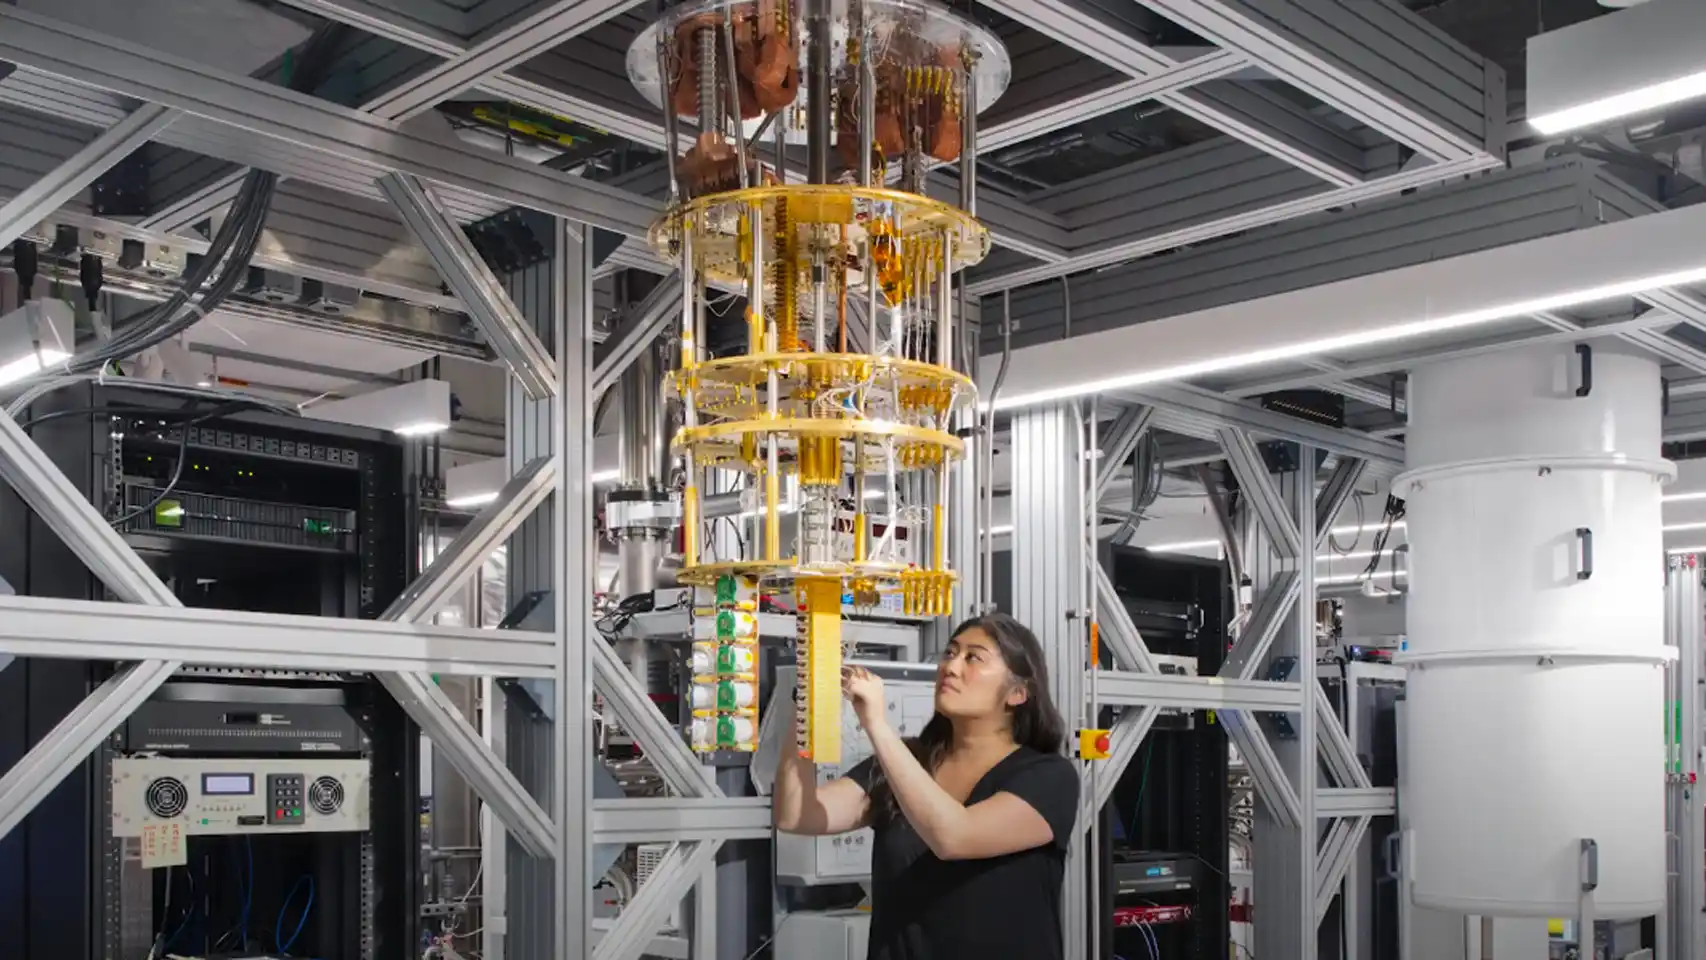
\includegraphics[width=10cm]{img/q.png}
\caption{Computadora cuantica de IBM}
\end{figure}

\subsection{Historia de la computacion cuantica}
\label{sec:org772fa63}
\autocite{Lopez_2023} Las computadoras cuánticas fueron propuestas en la década de 1980 por Richard Feynman y Yuri Manin. La intuición detrás de la computación cuántica surgió de lo que a menudo se consideraba una de las mayores vergüenzas de la física: un progreso científico notable enfrentado a la incapacidad de modelar incluso sistemas simples.

\subsection{Ventajsa}
\label{sec:orgf8c4941}
\begin{itemize}
\item \autocite{Marella_Parisa_2020} Puede resolver fácilmente problemas de optimización, como encontrar la mejor ruta y programar trenes y vuelos. También sería capaz de calcular 1 billón de movimientos en el ajedrez por segundo.

\item \autocite{Marella_Parisa_2020} Las computadoras cuánticas serán capaces de romper las técnicas de cifrado más seguras e inquebrantables. No obstante, también serán capaces de construir alternativas a prueba de hackeos.
\end{itemize}

\subsection{Desventajas}
\label{sec:org44afa83}
\begin{itemize}
\item \autocite{Marella_Parisa_2020} Aún no ha sido inventada por completo, ya que solo se están implementando partes y las personas aún están imaginando cómo sería.

\item \autocite{Marella_Parisa_2020} Es muy delicada y propensa a errores. Cualquier tipo de vibración afecta a las partículas subatómicas como átomos y electrones. Debido a esto, el ruido, las fallas e incluso los errores son posibles. Esto conduce a la "Descoherencia", que es una pérdida de coherencia en lo cuántico.
\end{itemize}

\section{Aplicaciones y Ejemplos}
\label{sec:orgdfd5559}
\subsection{Criptografia}
\label{sec:org8d91c57}
\autocite{Marella_Parisa_2020} Muchos elementos importantes de la seguridad informática. Esto se hace recorriendo todos los posibles factores utilizando computadoras convencionales, lo que lleva una cantidad significativa de tiempo. Nuevos algoritmos cuánticos (por ejemplo, el algoritmo de Shor) son capaces de hacerlo, y se desarrollarán algoritmos únicos adicionales. 

\subsection{Optimizacion}
\label{sec:org8f6badc}
\autocite{Marella_Parisa_2020} Las computadoras cuánticas son las mejores para resolver problemas de optimización. Hay muchos algoritmos cuánticos, de los cuales los algoritmos cuánticos de optimización pueden mejorar los problemas de optimización ya existentes que se resuelven actualmente con computadoras convencionales. 

\subsection{Inteligencia Artifial}
\label{sec:orgc6d7d92}
\autocite{Marella_Parisa_2020} La Inteligencia Artificial se basa en el procesamiento de conjuntos de datos grandes y complejos. Es responsable del aprendizaje, la inferencia y la comprensión. Aprende hasta que deja de cometer errores en su tarea. Las computadoras cuánticas pueden entrenar estos modelos en un conjunto de datos masivo sin caer en el tiempo exponencial.

\section{Datos de interés}
\label{sec:orgc5868d0}
\autocite{Arute_2019} Las computadoras cuánticas pueden resolver cualquier problema computacional que cualquier computadora clásica pueda resolver. De acuerdo con la tesis de Church-Turing, la inversa también es cierta: las computadoras clásicas pueden resolver todos los problemas de las computadoras cuánticas. Sin embargo, las computadoras cuánticas pueden resolver tales problemas en complejidades de tiempo razonable y exponencialmente menores, lo que también se conoce como "Supremacía Cuántica".

\section{Conclusion}
\label{sec:orgb3e5b06}
Las computadoras cuanticas a pesar de encontrarse en una etapa muy temprana de desarollo se muestran como una via hacia el futuro de la computacion y los medios de computacion tradicionales estan llegando a sus limites fisicos y cada vez se vuevlen mas costosos de utilizar para algunas aplicaciones.

\section{Fuentes}
\label{sec:org376ac05}
\printbibliography[heading=none]
\end{document}
